\documentclass[14pt]{beamer}
\usepackage[utf8]{inputenc}
\usepackage[T1]{fontenc}
\usepackage{lmodern}
\usepackage{amsmath}
\usepackage{amsfonts}
\usepackage{amssymb}
\usepackage{graphicx}
\usetheme{Madrid}
\usecolortheme{beaver}
\usepackage{tabulary}

\newcommand\e{\emph}
\newcommand\tb{\textbf}
\newcommand\un{\underline}
\newcommand\txt{\texttt}

\AtBeginSection[]{
	\begin{frame}
	\vfill
	\centering
	\begin{beamercolorbox}[sep=8pt,center,shadow=true,rounded=true]{title}
		\usebeamerfont{title}\insertsectionhead\par%
	\end{beamercolorbox}
	\vfill
\end{frame}
}

\begin{document}
\author[D. Christenson, J. Lin, and T. Makse] % (optional)
{Dino P. Christenson\inst{1}, Jennifer Lin\inst{2}, and Todd Makse\inst{3}}
\institute[] % (optional)
{
	\inst{1}%
	Faculty of Political Science\\
	Boston University
	\and
	\inst{2}%
	Undergraduate Student\\
	New College of Florida
	\and
	\inst{3}
	Faculty of Political Science\\
	Florida International University
}
\title[Demands for Representation]{Group Interests, Constituency Characteristics and Demands for Representation}
	%\subtitle{}
	%\logo{}
	\date[FPSA 2019]{Florida Political Science Association, March 2019}
	%\subject{}
	\setbeamercovered{transparent}
	\setbeamertemplate{navigation symbols}{}
	\begin{frame}[plain]
	\maketitle
\end{frame}

\begin{frame}
\frametitle{}
\begin{center}
	“If I hear 1 more person scream at a Rep., ‘I’m your boss!’, I’ll scream louder.
	Friends, each of us is 1/700,000th the boss of a congressman.”
\\\
	{\e {--- Larry Sabato on Twitter}}
\end{center}
\end{frame}

\begin{frame}
\frametitle{Guiding Questions}
\begin{enumerate}
	\item How does one's social identity influence their demands for representation?
	\item How does knowledge of the district's constituency characteristics influence one's demands for government responsiveness? 
\end{enumerate}
\end{frame}

\begin{frame}
\frametitle{Past Research}
\end{frame}

\begin{frame}
\footnotesize
\frametitle{Hypotheses}
\begin{enumerate}
	\item \tb{\e{Egocentric Hypothesis:}} As a representative's effort on behalf of groups with which the citizen identifies increases, the citizen's evaluation of the representative will become more positive. 
	\item \tb{\e{Proportionality Hypothesis:}} Citizens will expect that representatives expend effort on behalf of groups in proportion to their role in the constituency.
	\item \tb{\e{Heterogeneity Information Hypothesis:}} The link between representative effort, citizen identity and citizen evaluations will be attenuated by information about the heterogeneity of one’s constituency and strengthened by information about the homogeneity of one’s constituency. 
	\item \tb{\e{Size Information Hypothesis:}} The link between representative effort, citizen identity and citizen evaluations will be attenuated by information that the identity group is a small part of the constituency and strengthened by information that the identity group is a large part of the constituency. 
\end{enumerate}
\end{frame}

\section{Study 1}
\begin{frame}
\frametitle{Experimental Design}
\end{frame}

\begin{frame}
\frametitle{Distribution of Group Attachment}
\scriptsize
\begin{table}
	\centering
	\caption{Distribution of Group Attachment}
	\begin{tabulary}{\linewidth}{lc c c c}
		\\
		\hline 
		\tb{Group Interest}&\tb{Very Close}&\tb{Somewhat Close}&\tb{Not Close}&\tb{Partisan Gap*}\\
		\hline
		College Students&84\%&12\%&4\%&-0.01\\
		Small Business&26\%&44\%&30\%&0.17\\
		The Military& 23\%&37\%&40\%&0.22\\
		The Elderly&16\%&59\%&25\%&0.14\\
		The Poor&11\%&45\%&43\%&-0.22\\
		Farmers&10\%&30\%&60\%&0.17\\
		Unions&8\%&21\%&71\%&-0.12\\
		\hline
	\end{tabulary}\\
	*Partisan gap indicates the difference between Republicans and Democrats’ propensity to identify with the group. A score of 1.0 would indicate all Republicans very closely identify with the group and all Democrats do not feel close to the group, while a -1.0 would indicate the opposite.
\end{table}
\end{frame}

\begin{frame}
\frametitle{Experimental Condition Vignettes}
\scriptsize
\begin{table}
	\centering
	\begin{tabulary}{\linewidth}{p{5.5cm}p{5.5cm}}
	\\
	\hline
	\tb{Homogeneity Condition}&\tb{Heterogeneity Condition} \\
	\hline
	Based on the information provided, your member of Congress is Mike Turner, a member of the Republican Party. He has served in Congress since 2003. The Third District of Ohio is a largely urban district which is dominated by the city of Dayton; more than three-quarters of its population resides within Montgomery County. The district is heavily Republican: it has supported Republican presidential candidates in the last three elections, and Turner has not faced a competitive election since being elected to Congress. The district is also racially homogeneous: whites make up more than 80\% of the district’s residents, and this number rises to over 90\% outside of Dayton proper.&Based on the information provided, your member of Congress is Mike Turner, a member of the Republican Party. He has served in Congress since 2003. The Third District of Ohio stretches across large sections of southwestern Ohio, from the city of Dayton to rural counties east of Cincinnati. Although Dayton is the largest city in the district, a majority of its residents live in the Cincinnati media market. The district leans Republican in presidential and Congressional elections, but had a history of electing Democrats to Congress throughout the 1980s and 1990s, and the city of Dayton provides a strong based of Democratic support. The district ranks as one of the most racially diverse in the state of Ohio, with the city of Dayton almost evenly split between black and white residents.\\
	\hline
	\end{tabulary}
\end{table}
\end{frame}



\begin{frame}
\frametitle{Perceived Group Influence in Constituency}
\begin{figure}
	\centering
	{\includegraphics[width=.8\textwidth]{fig1color}}
\end{figure}
\end{frame}

\begin{frame}
\frametitle{Demands for Representational Effort}
\begin{figure}
	\centering
	{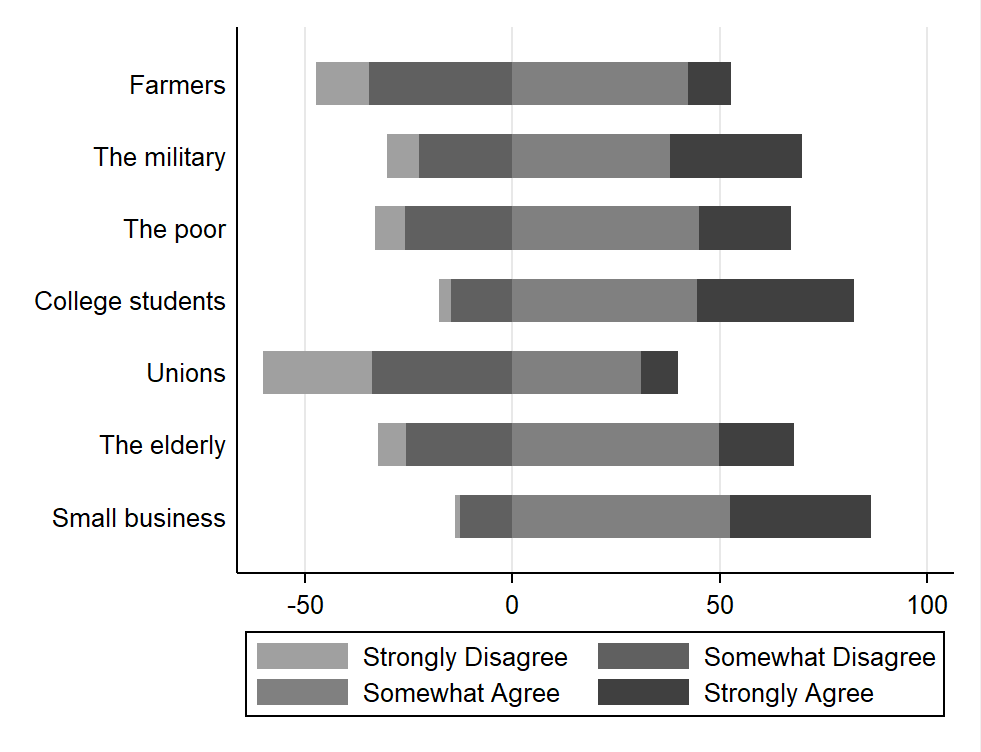
\includegraphics[width=.8\textwidth]{Figure2}}
\end{figure}
\end{frame}

%Generate Color version of this figure using code in Dropbox and replace in slide

\section{Study 2}
\begin{frame}
\frametitle{Experimental Design}
\end{frame}

\begin{frame}
\frametitle{Summary of Experimental Scenarios}
\tiny
\begin{table}
	\centering
	\def\arraystretch{1.5}
	\begin{tabulary}{\linewidth}{lCCC}
	\\
	\hline
	&\tb{Scenario 1}&\tb{Scenario 2}&\tb{Scenario 3}\\
	\hline
	Incumbent Decision&Voting for bill that would cut money for hypothetical university&Leading effort to pass financial reform bill that would cut student loan benefits&Accepting seat on Agriculture Committee in lieu of seat on Education Committee\\
	\hline
	Incumbent Defense&Other groups in district will benefit from the bill’s tax cut provisions&Bipartisanship is valuable; getting things done better than demanding the perfect bill&Agriculture is a large sector in the district; opponent pitting groups against each other\\
	\hline
	Constituency Trait Varied&Size of university, 
	\% of residents affiliated with the university&\% of college graduates in the district who have federal student loans&How rural district is; how large agricultural sector in district is\\
	\hline
	Condition 1&Largest university
	20\% of residents&50\% of graduates&75\% rural --
	Third largest agricultural sector in the country
\\
	\hline
	Condition 2&4th largest university
	1\% of residents&10\% of graduates&30\% rural
-- Agriculture is third largest sector in district
\\
	\hline
	\end{tabulary}
\end{table}
\end{frame}

\begin{frame}
\frametitle{Responses to Experiment Vignettes}
\scriptsize
\begin{table}
	\centering
	\begin{tabulary}{\linewidth}{Lccc}
	\\
	\hline
	&\tb{Scenario 1}&\tb{Scenario 2}&\tb{Scenario 3}\\
	&University Funding& Student Loans&Committee Work\\
	\hline
	\e{Incumbent Has Better Argument}&&&\\
	High Importance Condition&61.0\%&37.9\%&67.7\% \\
	Low Importance Condition&62.6\%&49.2\%&69.4\%\\
	Expected Difference (Sign)& ($-$)&($-$)&($+$)\\
	Observed Difference (S.E.)&$-0.2$ (0.06)&$-0.11$ (0.07) \# &$-0.02$ (0.06)\\
	N&225&225&225\\
	&&&\\
	\e{Vote for Incumbent}&&&\\
	High Importance Condition&51.7\%&42.1\%&61.2\%\\
	Low Importance Condition&50.5\%&41.5\%&65.4\%\\
	Expected Difference (Sign)& ($-$)&($-$)&($+$)\\
	Observed Difference&0.01 (0.07)&0.01 (0.07)&$-0,04$ (0.06)\\
	N&225&225&225\\
	\hline
	\end{tabulary}\\
Note: \# p $<$ 0.10; * p $<$ 0.05; ** p $<$ 0.01
\end{table}
\end{frame}

\section{General Discussion}
\begin{frame}
\frametitle{Conclusions}
\begin{center}
	\large
	\tb{Group Identities Guide Demands for Responsiveness} \\
	\smallskip
	\normalsize 
	Voters favor representatives who cater to their most salient social identities
\end{center}
\begin{itemize}
	\small
	\item Study 1: Closeness to group influences perceptions of what warrants representation 
	\item Study 2: District composition does not do much to influence evaluations demands for representation
\end{itemize}
\end{frame}

\begin{frame}
\frametitle{Future Directions}
\begin{itemize}
	\item Observing results via observational methods 
	\begin{itemize}
		\item Campaigns
		\item Legislative Behavior
		\item Outcome of Future Elections
	\end{itemize}
\end{itemize}
\end{frame}

\section{Questions?}



\end{document}